\documentclass[aspectratio=169,11pt]{beamer}

% common_setting.tex
% Shared preamble for the five PSPDE2026 workshop beamer decks (00-04).
% \input this right after \documentclass in each deck.
% Requires xelatex (fontspec/unicode-math need XeTeX or LuaTeX, not pdflatex).

% Fonts
\usepackage{fontspec}
\usepackage{unicode-math}
\setmainfont{Liberation Sans}
\setsansfont{Liberation Sans}
\setmonofont{Liberation Mono}[Scale=0.85]
\setmathfont{Latin Modern Math}

% Theme and colors
\usetheme{moloch}
\molochset{
  block=fill,
  progressbar=frametitle,
  sectionpage=progressbar,
}
\setbeamertemplate{page number in head/foot}[totalframenumber]

% Graphics
\usepackage{graphicx}
\graphicspath{{./figures/}}

% Tables
\usepackage{booktabs}
\usepackage{tabularx}

% Unnumbered captions without the "Figure:" label prefix
\usepackage{caption}
\captionsetup{labelformat=empty}

% Code listings
\usepackage{listings}
\usepackage{xcolor}
\definecolor{codebg}{RGB}{245,245,245}
% moloch's own accent colors, aliased under their original Metropolis names
\colorlet{mAlertFg}{mLightBrown}
\colorlet{mExampleFg}{mLightGreen}
\lstdefinestyle{python}{
  language=Python,
  basicstyle=\ttfamily\scriptsize,
  keywordstyle=\color{mAlertFg}\bfseries,
  commentstyle=\color{mExampleFg}\itshape,
  stringstyle=\color{mExampleFg!70!black},
  backgroundcolor=\color{codebg},
  rulecolor=\color{black!15},
  frame=single,
  breaklines=true,
  showstringspaces=false,
  columns=fullflexible,
  numbers=none
}
\lstdefinestyle{shell}{
  basicstyle=\ttfamily\scriptsize,
  backgroundcolor=\color{codebg},
  rulecolor=\color{black!15},
  frame=single,
  breaklines=true,
  columns=fullflexible
}


% Title information
\title[apsg advanced]{Advanced Structural and Tensor Analysis}
\subtitle{Block 2 --- Modern Workflow in Geology}
\author[O.\ Lexa]{Ondrej Lexa}
\institute[Charles University]{
  Institute of Petrology and Structural Geology (IPSG)\\
  Charles University, Prague, Czechia
}
\date{8 October 2026}

\begin{document}

\begin{frame}[plain]
  \titlepage
\end{frame}

\begin{frame}{This Block (11:15--12:30)}
  \begin{block}{Objective}
    Functions that would take hours by hand: kinematic analysis of faults,
    finite strain and progressive deformation, stress, and stress inversion.
  \end{block}
  \vspace{0.3cm}
  \begin{enumerate}
    \item Fault-slip data: Angelier and Hoeppner plots, P/T axes, right dihedra
    \item Deformation gradient, strain ellipsoid, progressive deformation
    \item Superposition of deformations
    \item Strain analysis from markers: Rf/φ, Robin mean ellipse/ellipsoid
    \item Stress tensor and stress inversion
  \end{enumerate}
  \vspace{0.2cm}
  \small Notebook: \texttt{notebooks/02\_apsg\_advanced.ipynb}.
  Tensors combine with \texttt{@} --- never \texttt{*}.
\end{frame}

\section{Kinematics and Faults}

\begin{frame}[fragile]{Fault-Slip Data}
  \begin{columns}[T]
    \begin{column}{0.55\textwidth}
      \begin{lstlisting}[style=python]
faults = faultset.from_csv("data/mele.csv")
# columns: fazi, finc, lazi, linc, sense
# or: pd.read_csv("data/mele.csv").fault()

s = StereoNet(title="Angelier plot")
s.fault(faults)
s.show()

s = StereoNet(title="Hoeppner plot")
s.hoeppner(faults)
      \end{lstlisting}
      \small Sense: \texttt{1}/\texttt{"n"} normal, \texttt{-1}/\texttt{"r"} reverse,
      \texttt{"s"} sinistral, \texttt{"d"} dextral.
    \end{column}
    \begin{column}{0.42\textwidth}
      \begin{figure}
        \centering
        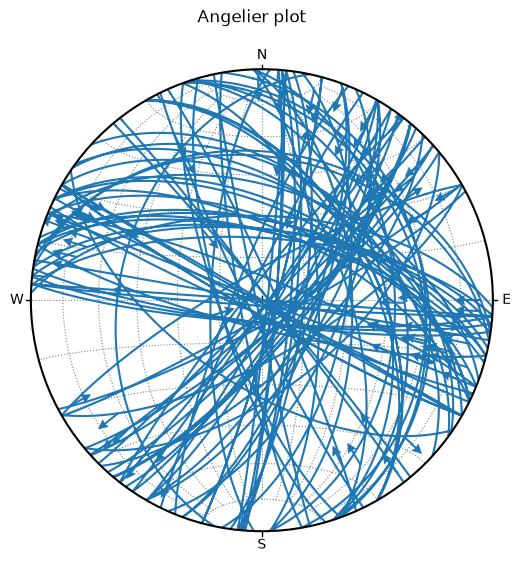
\includegraphics[width=\textwidth,height=0.68\textheight,keepaspectratio]{nb_angelier.png}
        \caption*{\footnotesize 94 faults, Angelier plot}
      \end{figure}
    \end{column}
  \end{columns}
\end{frame}

\begin{frame}[fragile]{Right Dihedra}
  \begin{columns}[T]
    \begin{column}{0.36\textwidth}
      \begin{lstlisting}[style=python]
f = faults[62]       # F:120/68-49/38 R
s = StereoNet()
s.dihedra(f)         # extensional dihedra
s.fault(f)
s.line(f.p, color="r", label="P")
s.line(f.t, color="b", label="T")

s = StereoNet()
s.dihedra(faults)    # all 94 faults
      \end{lstlisting}
      \small Fault plane + auxiliary plane split the sphere into two compressional
      and two extensional dihedra. Where many faults overlap, the shading is
      darkest (σ3); unshaded areas are the σ1 candidates.
    \end{column}
    \begin{column}{0.62\textwidth}
      \begin{figure}
        \centering
        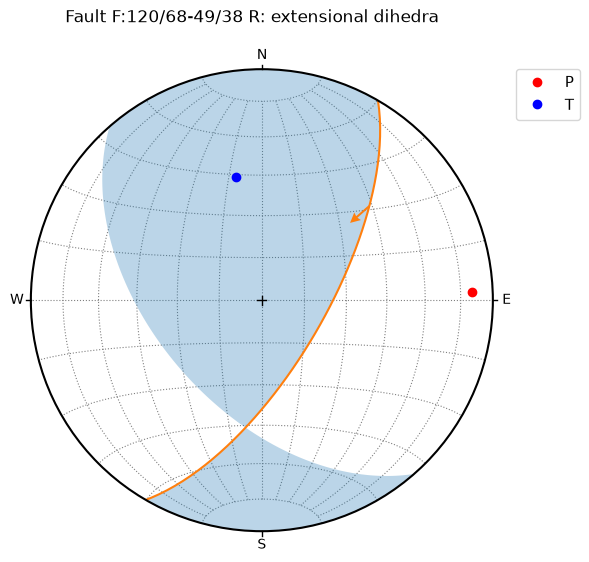
\includegraphics[width=0.5\textwidth,height=0.7\textheight,keepaspectratio]{nb_dihedra_fault.png}%
        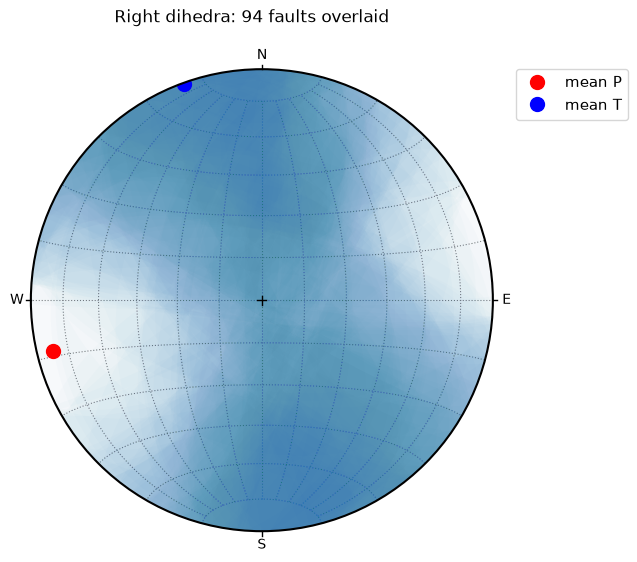
\includegraphics[width=0.5\textwidth,height=0.7\textheight,keepaspectratio]{nb_dihedra_set.png}
      \end{figure}
    \end{column}
  \end{columns}
\end{frame}

\begin{frame}[fragile]{P/T Axes and Right-Dihedra Count}
  \begin{columns}[T]
    \begin{column}{0.5\textwidth}
      \begin{lstlisting}[style=python]
P, T = faults.p, faults.t     # LineationSets
P.ortensor().eigenlins(0)     # L:256/8

g = StereoGrid()
g.angmech(faults)             # Angelier-Mechler
s = StereoNet()
s.contour(g, clip=False, colorbar=True)
print(g)  # max 90 at L:268/2, min -84 at L:167/11
      \end{lstlisting}
      \small Model-free first look at the kinematics: every direction is
      counted as compressional (+) or extensional (--) for each fault.
    \end{column}
    \begin{column}{0.47\textwidth}
      \begin{figure}
        \centering
        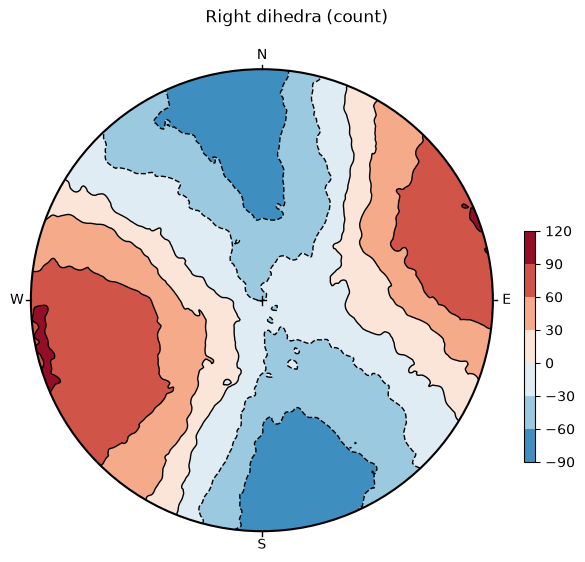
\includegraphics[width=\textwidth,height=0.68\textheight,keepaspectratio]{nb_dihedra.png}
      \end{figure}
    \end{column}
  \end{columns}
\end{frame}

\section{Finite Strain}

\begin{frame}[fragile]{Deformation Gradient}
  \begin{columns}[T]
    \begin{column}{0.55\textwidth}
      \begin{lstlisting}[style=python]
F = defgrad.from_comp(xx=2, zz=0.5, xz=1)
F @ vec("x")          # deformed vector
F.R, F.U              # rotation, stretch
defgrad.from_ratios(Rxy=2, Ryz=3)

Lr = linset.random_fisher(position=lin(0, 90),
                          kappa=1, n=300)
s = StereoNet()
s.line(Lr, color="0.7", ms=2)
s.line(Lr.transform(F), color="k", ms=2)
      \end{lstlisting}
      \small Any feature or set can be \texttt{.transform(F)}-ed --- planes are
      handled correctly through their poles.
    \end{column}
    \begin{column}{0.42\textwidth}
      \begin{figure}
        \centering
        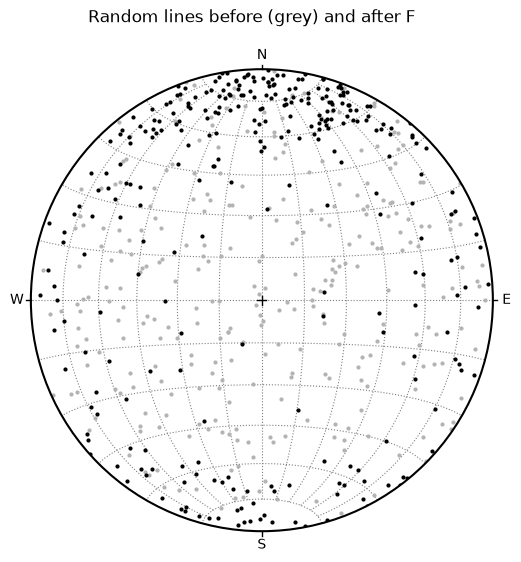
\includegraphics[width=\textwidth,height=0.68\textheight,keepaspectratio]{nb_defgrad_lines.png}
      \end{figure}
    \end{column}
  \end{columns}
\end{frame}

\begin{frame}[fragile]{Strain Ellipsoid}
  \begin{lstlisting}[style=python]
B = ellipsoid.from_defgrad(F)       # Finger tensor B = F F^T
B.Rxy, B.Ryz, B.k, B.lode           # 2.25, 2.25, 1.00, 0.00
B.eigenlins()                       # X, Y, Z directions: L:0/6, L:270/0, L:180/84
V = B.defgrad()                     # symmetric stretch V, the same as F.V
np.allclose(V @ F.R, F)             # True: F = V R, rotation R is not in B
  \end{lstlisting}
  \vspace{0.3cm}
  \begin{itemize}
    \item Shape descriptors: \texttt{Rxy}, \texttt{Ryz}, Flinn \texttt{k},
          Lode \texttt{lode}, \texttt{P\_j}, \texttt{T}, \ldots
    \item Principal directions: \texttt{B.eigenlins()} (X, Y, Z),
          \texttt{B.eigenfols()} (principal planes)
    \item Fabric plots: \texttt{FlinnPlot}, \texttt{RamsayPlot},
          \texttt{VollmerPlot}, \texttt{HsuPlot} --- \texttt{.point(E)} or \texttt{.path(Eset)}
    \item The same plots take orientation tensors (\texttt{ortensor}) of measured fabrics
  \end{itemize}
\end{frame}

\begin{frame}[fragile]{Progressive Deformation}
  \begin{columns}[T]
    \begin{column}{0.55\textwidth}
      \begin{lstlisting}[style=python]
Lss = velgrad.from_comp(xz=1)     # simple shear
Lss.kinematic_vorticity           # Wk = 1.0
Lss.defgrad(time=2)               # F = exp(L t)

flows = {
 "constriction": velgrad.from_comp(
                   xx=1, yy=-0.5, zz=-0.5),
 "plane strain": velgrad.from_comp(xx=1, zz=-1),
 "flattening":   velgrad.from_comp(
                   xx=0.5, yy=0.5, zz=-1)}
fp = FlinnPlot()
for name, L in flows.items():
    E = ellipsoidset([ellipsoid.from_defgrad(
          L.defgrad(time=t)) for t in times])
    fp.path(E, label=name, marker=".")
      \end{lstlisting}
    \end{column}
    \begin{column}{0.42\textwidth}
      \begin{figure}
        \centering
        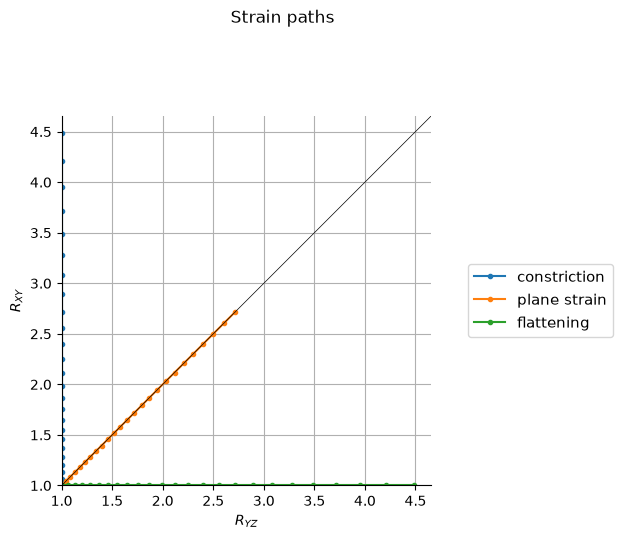
\includegraphics[width=\textwidth,height=0.68\textheight,keepaspectratio]{nb_flinn_paths.png}
      \end{figure}
    \end{column}
  \end{columns}
\end{frame}

\begin{frame}[fragile]{Rotating Fabrics during Flow}
  \begin{columns}[T]
    \begin{column}{0.5\textwidth}
      \begin{lstlisting}[style=python]
L0 = linset.random_fisher(position=lin(45, 30),
                          kappa=50, n=50)
s = StereoNet()
for t in [0, 0.5, 1, 2, 4]:
    s.line(L0.transform(Lss.defgrad(time=t)),
           ms=2, label=f"t = {t}")
s.show()
      \end{lstlisting}
      \small Lineations progressively rotate towards the shear direction
      ($x$ = north) --- the basis for interpreting stretching lineations in
      shear zones.
    \end{column}
    \begin{column}{0.47\textwidth}
      \begin{figure}
        \centering
        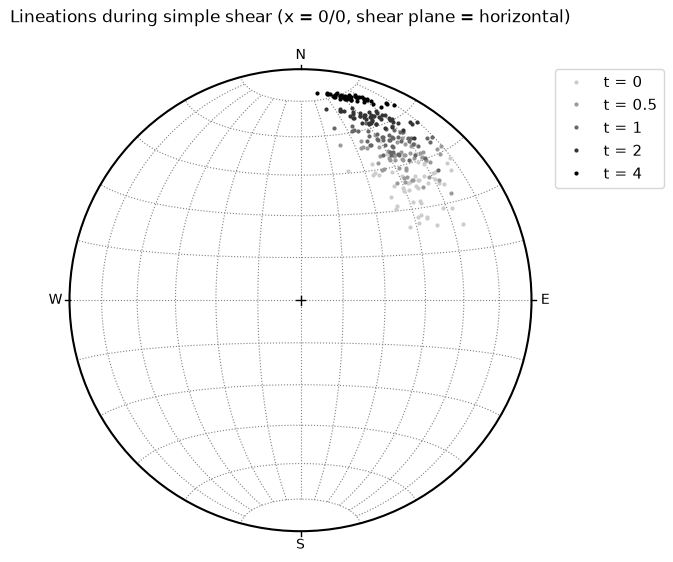
\includegraphics[width=\textwidth,height=0.68\textheight,keepaspectratio]{nb_simple_shear_lines.png}
      \end{figure}
    \end{column}
  \end{columns}
\end{frame}

\begin{frame}[fragile]{Superposition of Deformations}
  \begin{lstlisting}[style=python]
F1 = defgrad.from_comp(xx=2, zz=0.5)               # D1: pure shear
F2 = rotation.from_axisangle(lin(0, 90), 60)       # rigid rotation about vertical
F3 = defgrad.from_comp(xy=1)                       # D2: simple shear

ellipsoid.from_defgrad(F3 @ F2 @ F1)   # D1 -> rot -> D2:  Rxy=5.23 Ryz=1.24
ellipsoid.from_defgrad(F1 @ F2 @ F3)   # D2 -> rot -> D1:  Rxy=1.32 Ryz=2.47
  \end{lstlisting}
  \vspace{0.3cm}
  \begin{block}{Order matters}
    Finite deformations combine by matrix multiplication with the
    \textbf{later event on the left}: $\mathbf{F} = \mathbf{F}_2 \cdot \mathbf{F}_1$.
    Matrix products do not commute --- the same two events in a different
    order give a different finite strain.
  \end{block}
\end{frame}

\section{Strain Analysis}

\begin{frame}[fragile]{Strain from Markers: Rf/φ}
  \begin{columns}[T]
    \begin{column}{0.55\textwidth}
      \begin{lstlisting}[style=python]
pebbles0 = ellipseset([       # 80 random markers
    ellipse.from_ratio(R=r)
           .transform(rotation2.from_angle(p))
    for r, p in zip(Ri, phi_i)])  # Ri 1-2.5
F = defgrad2.from_comp(xy=1.5)    # simple shear
pebbles = pebbles0.transform(F)

ellipse.from_defgrad(F)  # true: ar 4, ori 26.6
pebbles.rfphi()          # Rs = 4.34, phi = 27.0
pebbles.robin()          # Rs = 4.34, phi = 27.0
pebbles.ar.mean()        # 4.72 - biased
      \end{lstlisting}
      \small \texttt{rfphi()}: vector mean of ln Rf at 2φ.
      \texttt{robin()}: log-matrix mean (Robin 1977) --- identical in 2D.
    \end{column}
    \begin{column}{0.42\textwidth}
      \begin{figure}
        \centering
        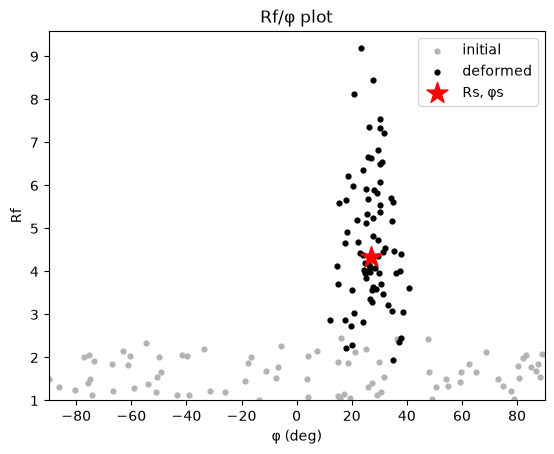
\includegraphics[width=\textwidth,height=0.68\textheight,keepaspectratio]{nb_rfphi.png}
      \end{figure}
    \end{column}
  \end{columns}
\end{frame}

\begin{frame}[fragile]{Mean Strain Ellipsoid (Robin 1977)}
  \begin{lstlisting}[style=python]
stations = ellipsoidset([...])  # 15 strain ellipsoids, axes scattered by ~15 deg
Emean = stations.robin()        # Rxy=2.35 Ryz=1.50 k=2.70 volume=1.00
ellipsoid(np.mean([np.asarray(E) for E in stations], axis=0))   # volume=1.10
fp = FlinnPlot()
fp.point(stations, color="0.5"); fp.point(Emean, color="r", ms=10)
s = StereoNet()
s.tensor(stations, planes=False, ms=4)     # principal axes of all stations
  \end{lstlisting}
  \vspace{-0.3cm}
  \begin{figure}
    \centering
    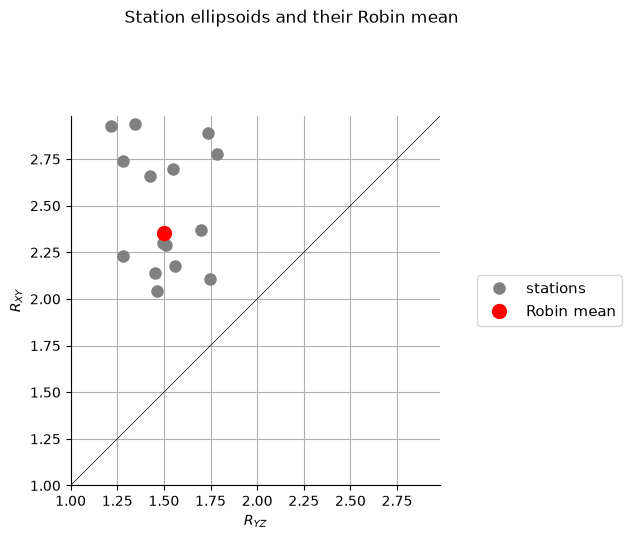
\includegraphics[height=0.48\textheight,keepaspectratio]{nb_robin_flinn.png}
    \hspace{0.3cm}
    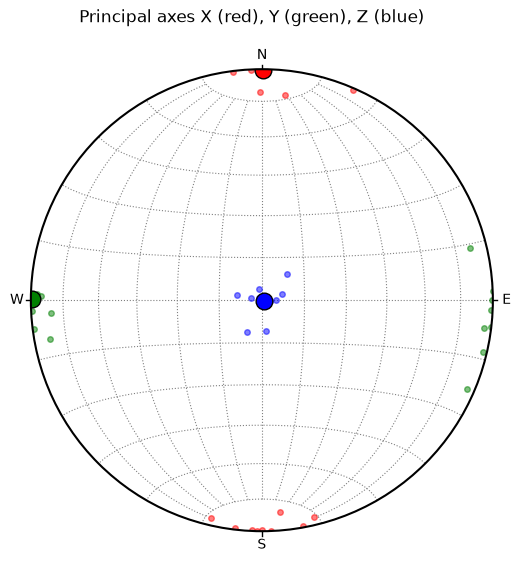
\includegraphics[height=0.48\textheight,keepaspectratio]{nb_robin_axes.png}
  \end{figure}
\end{frame}

\section{Stress}

\begin{frame}[fragile]{Stress Tensor}
  \begin{columns}[T]
    \begin{column}{0.53\textwidth}
      \begin{lstlisting}[style=python]
S = stress.from_comp(xx=8, yy=5, zz=1)
S.sigma1, S.sigma2, S.sigma3   # 8, 5, 1
lin(S.sigma1dir)               # L:0/0
S.shape_ratio                  # 0.43

n = fol(120, 60)
S.normal_stress(n)             # 4.56
S.shear_stress(n)              # 2.34
S.slip_tendency(n)             # 0.51
S.fault(n)          # predicted slip (Wallace-Bott)

rot = rotation.from_axisangle(lin(120, 50), 40)
Sr = S.transform(rot)          # oblique axes
lin(Sr.sigma1dir)              # L:210/25
g = StereoGrid()
g.apply_func(Sr.slip_tendency)
StereoNet().contour(g, colorbar=True)
      \end{lstlisting}
      \small Geological convention: \textbf{compression positive}.
    \end{column}
    \begin{column}{0.44\textwidth}
      \begin{figure}
        \centering
        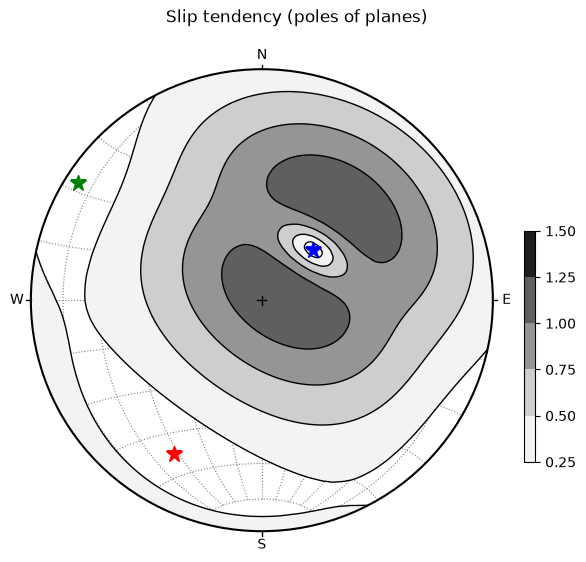
\includegraphics[width=\textwidth,height=0.68\textheight,keepaspectratio]{nb_slip_tendency.png}
      \end{figure}
    \end{column}
  \end{columns}
\end{frame}

\begin{frame}[fragile]{Stress Inversion --- Test First}
  \begin{lstlisting}[style=python]
synthetic = faultset([S.fault(n) for n in vecset.gss(n=200)])
Sinv = synthetic.stress_inversion()
# true     sigma1: L:0/0  R = 0.43
# inverted sigma1: L:0/0  R = 0.41
  \end{lstlisting}
  \vspace{0.2cm}
  \begin{itemize}
    \item \texttt{faultset.stress\_inversion()} --- linear least-squares method of
          Michael (1984): the reduced stress tensor that best explains all
          striations at once
    \item Faults generated from a \emph{known} tensor must return it ---
          a habit worth keeping for any black-box method
  \end{itemize}
\end{frame}

\begin{frame}[fragile]{Stress Inversion --- Real Data}
  \begin{columns}[T]
    \begin{column}{0.53\textwidth}
      \begin{lstlisting}[style=python]
Smele = faults.stress_inversion()
lin(Smele.sigma1dir)   # L:244/11
lin(Smele.sigma3dir)   # L:335/4
Smele.shape_ratio      # 0.59

misfit = faults.angular_misfit(Smele)
np.median(misfit)      # 22.9 deg

boot = faults.stress_inversion(   # Stress3Set
           bootstrap=True, n=100)
s = StereoNet()
s.hoeppner(faults, color="0.6")
s.tensor(boot, planes=False, ms=2, alpha=0.4)
s.stress(Smele, mec="k")
      \end{lstlisting}
    \end{column}
    \begin{column}{0.44\textwidth}
      \begin{figure}
        \centering
        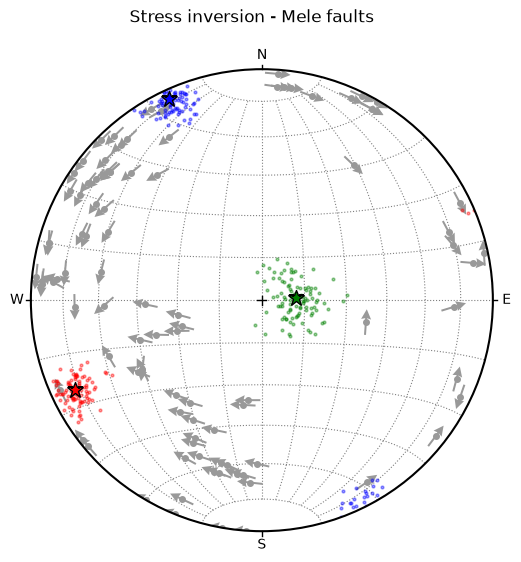
\includegraphics[width=\textwidth,height=0.68\textheight,keepaspectratio]{nb_stress_inversion.png}
        \caption*{\footnotesize bootstrap $\sigma_{1,2,3}$: red, green, blue}
      \end{figure}
    \end{column}
  \end{columns}
\end{frame}

\section{Hands-on}

\begin{frame}{Hands-on Exercise}
  \begin{columns}[T]
    \begin{column}{0.55\textwidth}
      \small
      \textbf{A. Progressive deformation and superposition}
      \begin{enumerate}
        \item 50 lineations around \texttt{lin(90, 20)}
        \item D1: pure shear \texttt{velgrad.from\_comp(xx=-1, zz=1)}, \texttt{time=0.5};
              D2: simple shear \texttt{from\_comp(xy=1)}, \texttt{time=1}
        \item Plot initial / D1 / D1+D2; ellipsoid of the total --- does swapping
              the order matter?
      \end{enumerate}
      \textbf{B. Brittle structures}
      \begin{enumerate}
        \setcounter{enumi}{3}
        \item Keep Mele faults with misfit $<$ 30\textdegree{} and invert again
        \item Save Angelier plot + principal stresses as PDF
      \end{enumerate}
    \end{column}
    \begin{column}{0.42\textwidth}
      \begin{figure}
        \centering
        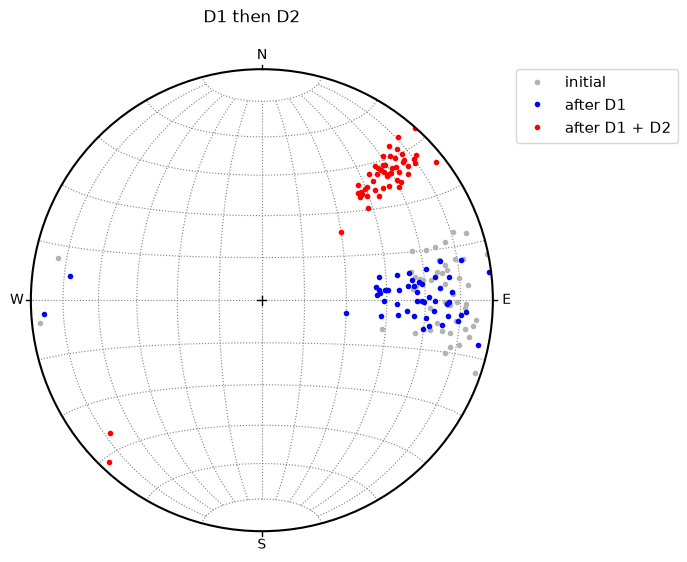
\includegraphics[width=\textwidth,height=0.7\textheight,keepaspectratio]{nb_superposition.png}
        \caption*{\footnotesize Part A result (solution in the notebook)}
      \end{figure}
    \end{column}
  \end{columns}
\end{frame}

\section{Recap}

\begin{frame}{Recap}
  \centering
  \small
  \begin{tabular}{ll}
    \toprule
    \textbf{Task} & \textbf{Code} \\
    \midrule
    Fault data \& plots & \texttt{faultset.from\_csv}, \texttt{s.fault}, \texttt{s.hoeppner} \\
    Kinematics & \texttt{fs.p}, \texttt{fs.t}, \texttt{s.dihedra(fs)}, \texttt{StereoGrid().angmech(fs)} \\
    Finite strain & \texttt{defgrad}, \texttt{F.R}, \texttt{F.U}, \texttt{ellipsoid.from\_defgrad(F)} \\
    Flow & \texttt{velgrad}, \texttt{L.defgrad(time=t)}, \texttt{L.kinematic\_vorticity} \\
    Superposition & \texttt{F2 @ F1} (later event on the left) \\
    Strain markers & \texttt{ellipseset.rfphi()}, \texttt{.robin()}, \texttt{ellipsoidset.robin()} \\
    Stress & \texttt{stress.from\_comp}, \texttt{.sigma1dir}, \texttt{.shear\_stress(n)}, \texttt{.fault(n)} \\
    Inversion & \texttt{fs.stress\_inversion()}, \texttt{fs.angular\_misfit(S)}, \texttt{bootstrap=True} \\
    \bottomrule
  \end{tabular}

  \vspace{0.5cm}
  \Large After lunch: petrological data with \texttt{petropandas}
\end{frame}

\end{document}
